\documentclass[10pt, dvipdfmx]{beamer}
\AtBeginDvi{\special{pdf:tounicode 90ms-RKSJ-UCS2}}
\usetheme{default}
\usefonttheme{professionalfonts}
\usepackage{helvet}
\usepackage{txfonts}
\usepackage{moreverb}
\renewcommand{\familydefault}{\sfdefault}
\renewcommand{\kanjifamilydefault}{\gtdefault}
\setbeamertemplate{caption}[numbered]

\title{レーザーカッターでガワを作る}
\author{}
\institute[所属]{}
\date{\today}

\uselanguage{japanese}
\languagepath{japanese}

\begin{document}
    \begin{frame}[plain]
        \frametitle{}
	    \titlepage
    \end{frame}

    \begin{frame}
        \frametitle{Contents}
        \tableofcontents
    \end{frame}

%-----------------------------------------------------------
    \section{効率よく工作機械を使うには}
        \begin{frame}
            \frametitle{ネットでデータ配布}
            \begin{block}{さまざまなデータ共有サービス}
                \begin{itemize}
                    \item thingivers(ehttp://www.thingiverse.com/)
                    \item Adafruit(https://learn.adafruit.com/all-about-laser-cutters/overview)
                \end{itemize}
            \end{block}
        \end{frame}

        \begin{frame}
            \frametitle{Generator}
            \begin{block}{世の中に出回っているGenerator}
                \begin{itemize}
                    \item projectGenerator(openFrameworks)
                    \item SkateBoardDeckGenerator
                    \item chair Generator
                    \item NormalBoxTool
                \end{itemize}
            \end{block}
        \end{frame}

%-----------------------------------------------------------
    \section{各ツール紹介}
        \begin{frame}
            \frametitle{projectGenerator(openFrameworks)}
            \tiny
            \begin{columns}[c]
                \begin{column}{0.50\textwidth}
                    \begin{figure}[htb]
                        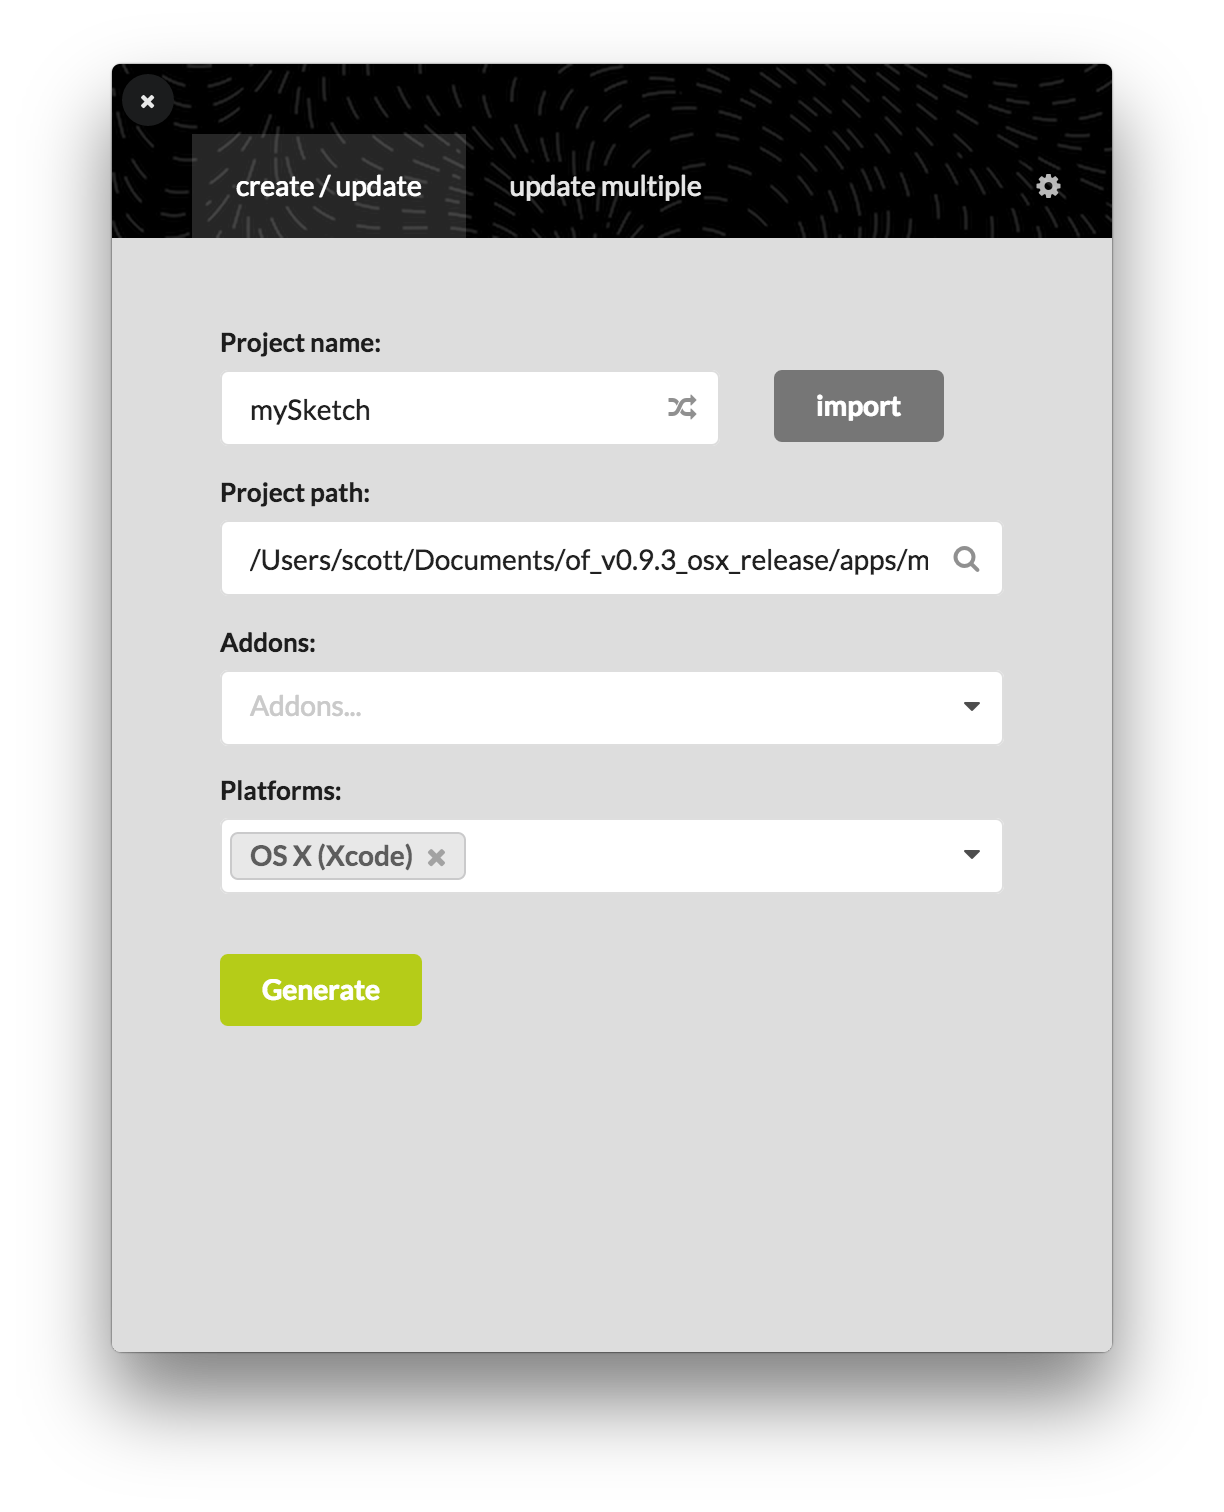
\includegraphics[width=\columnwidth]{images/01.png}
                        \caption{projectGenerator UI}
                        \label{fig:01}
                    \end{figure}
                \end{column}
                \begin{column}{0.50\textwidth}
                    \begin{block}{手順}
                        \begin{itemize}
                            \item Project nameを変える
                            \item Project pathを変える
                            \item Addonなど加える
                            \item Generateする
                        \end{itemize}
                    \end{block}
                \end{column}
            \end{columns}
        \end{frame}

        \begin{frame}
            \frametitle{SkateboardGenerator}
            \tiny
            \begin{columns}[c]
                \begin{column}{0.50\textwidth}
                    \begin{figure}[htb]
                        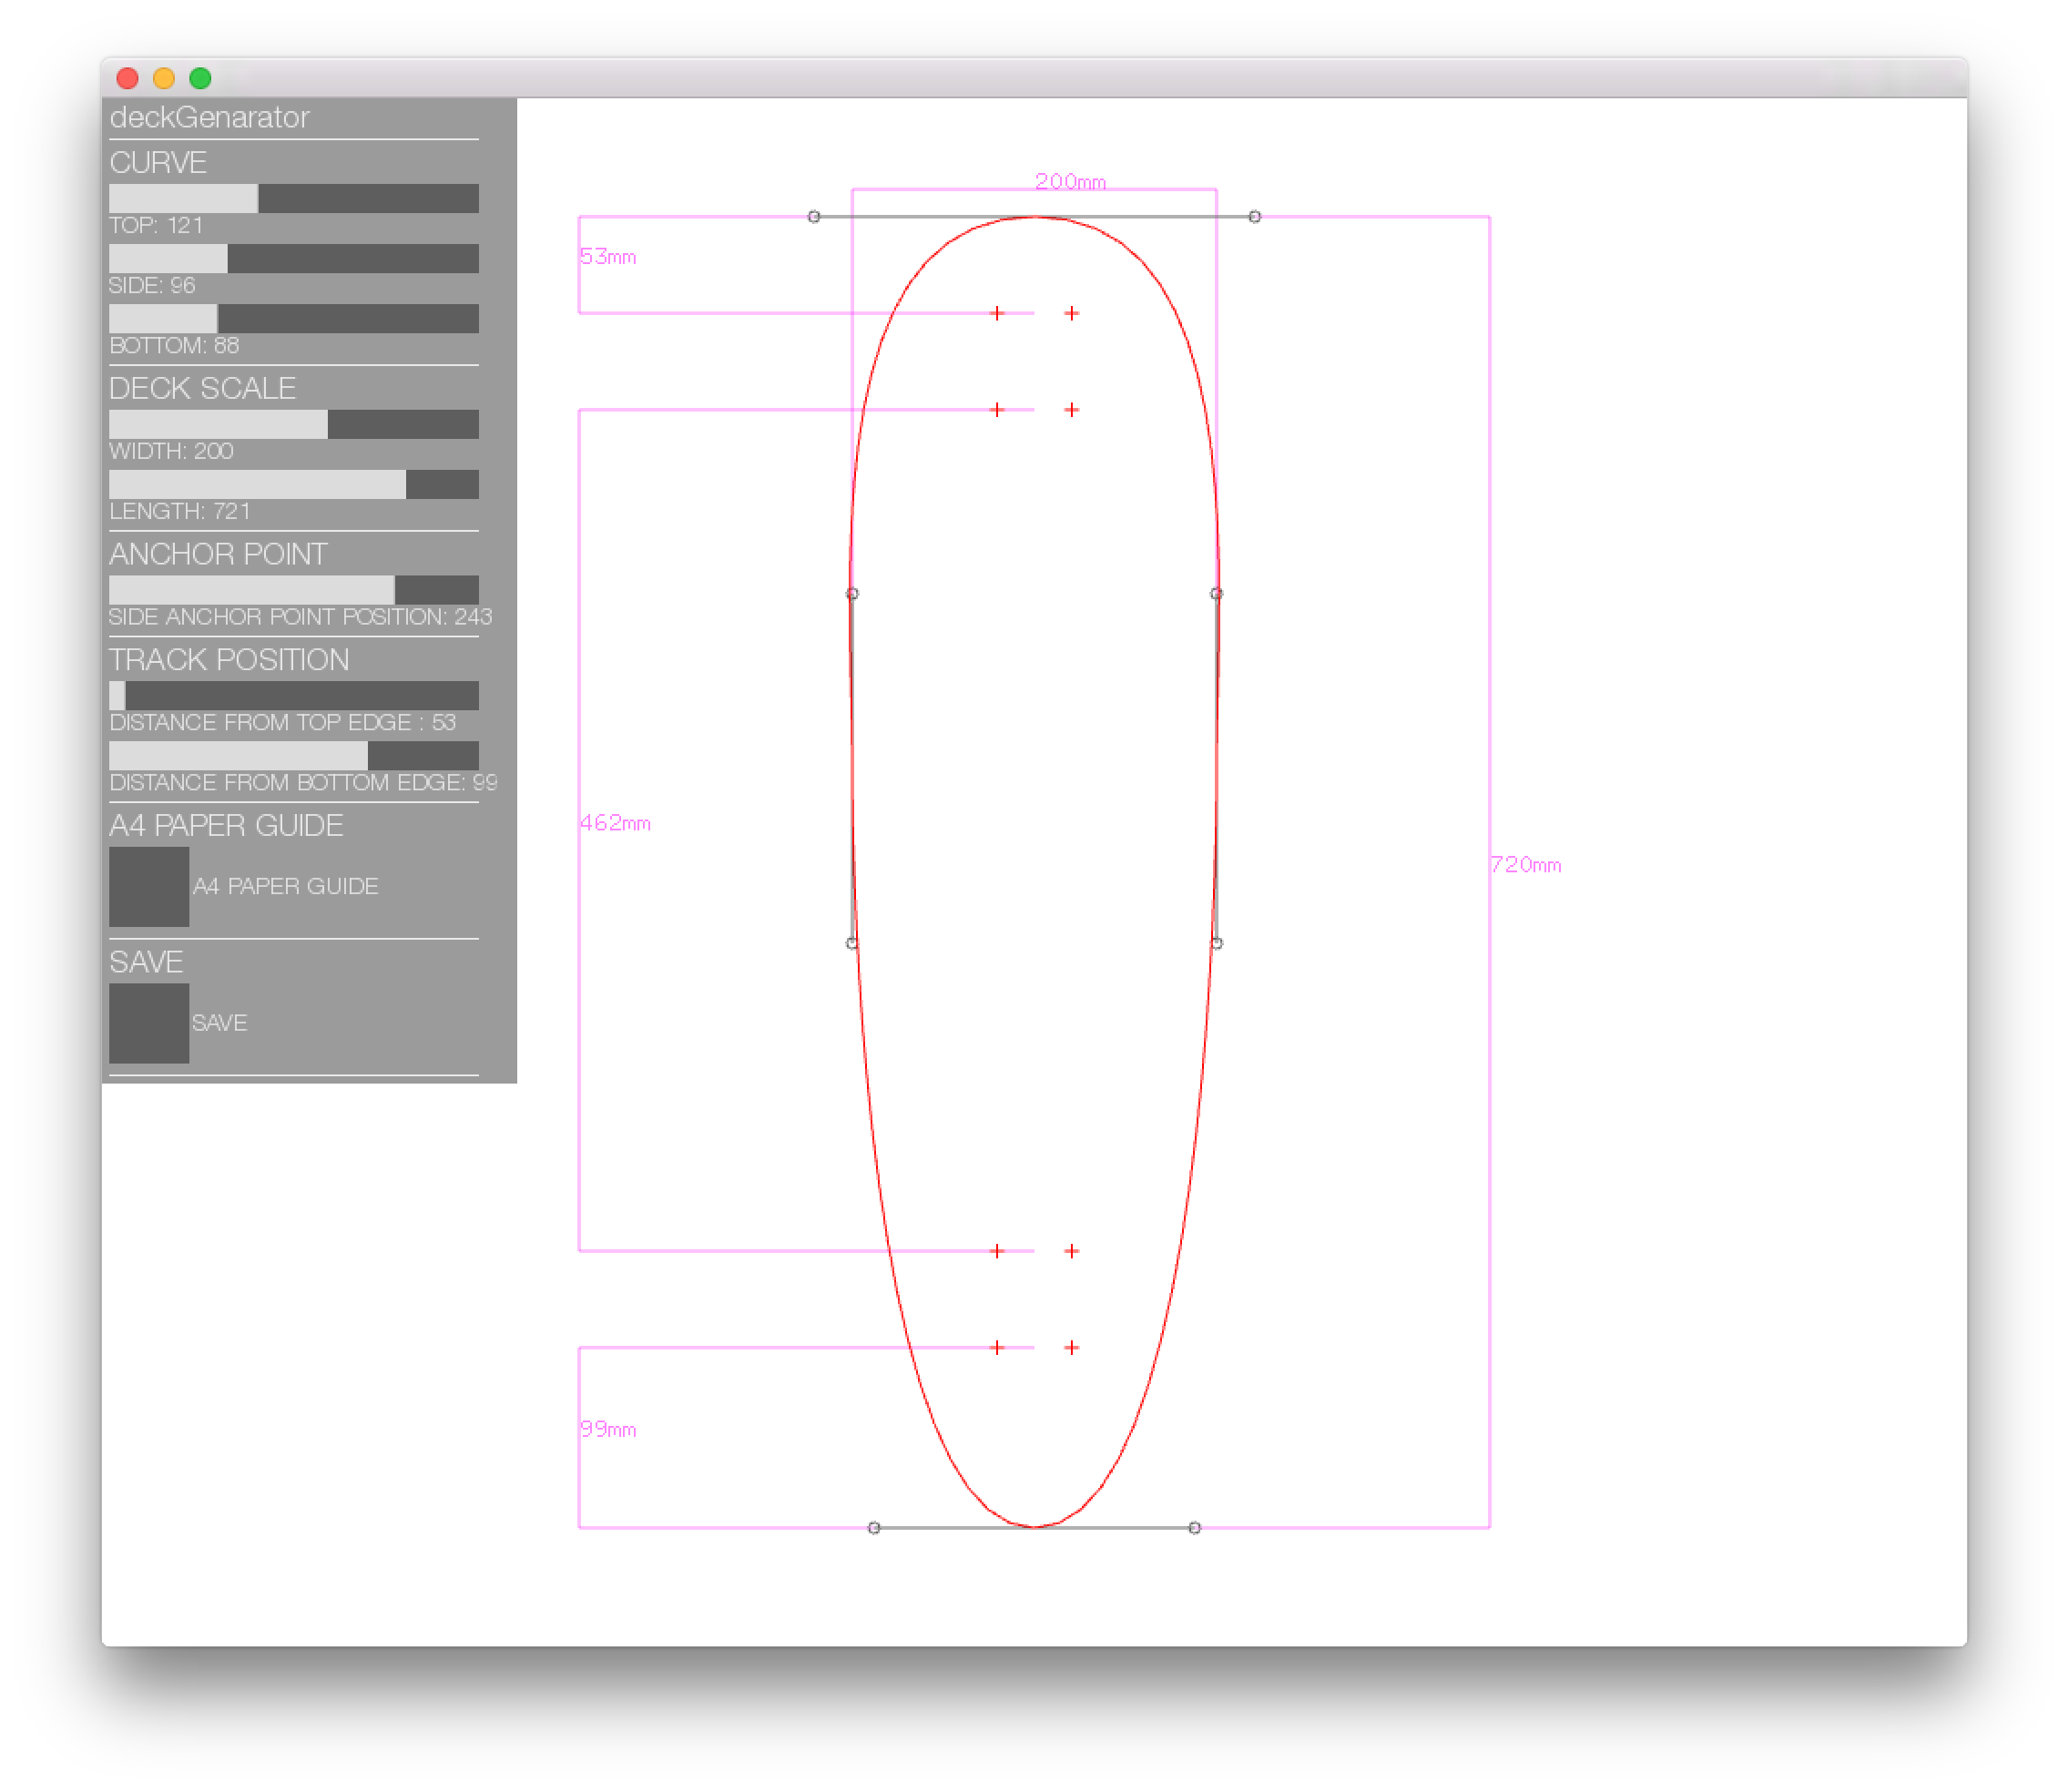
\includegraphics[width=\columnwidth]{images/02.png}
                        \caption{SkateBoardDeckGenerator UI}
                        \label{fig:01}
                    \end{figure}
                \end{column}
                \begin{column}{0.50\textwidth}
                    \begin{block}{手順}
                        \begin{itemize}
                            \item パラメーターをスライドする
                            \item SAVEボタンを押してパスデータを保存する
                            \item レーザーカッターやショップボットで切る
                            \item http://skateboarddeckgenerator.scottallen.ws/
                        \end{itemize}
                    \end{block}
                \end{column}
            \end{columns}
        \end{frame}

        \begin{frame}
            \frametitle{chairGenerator}
            \tiny
            \begin{columns}[c]
                \begin{column}{0.50\textwidth}
                    \begin{figure}[htb]
                        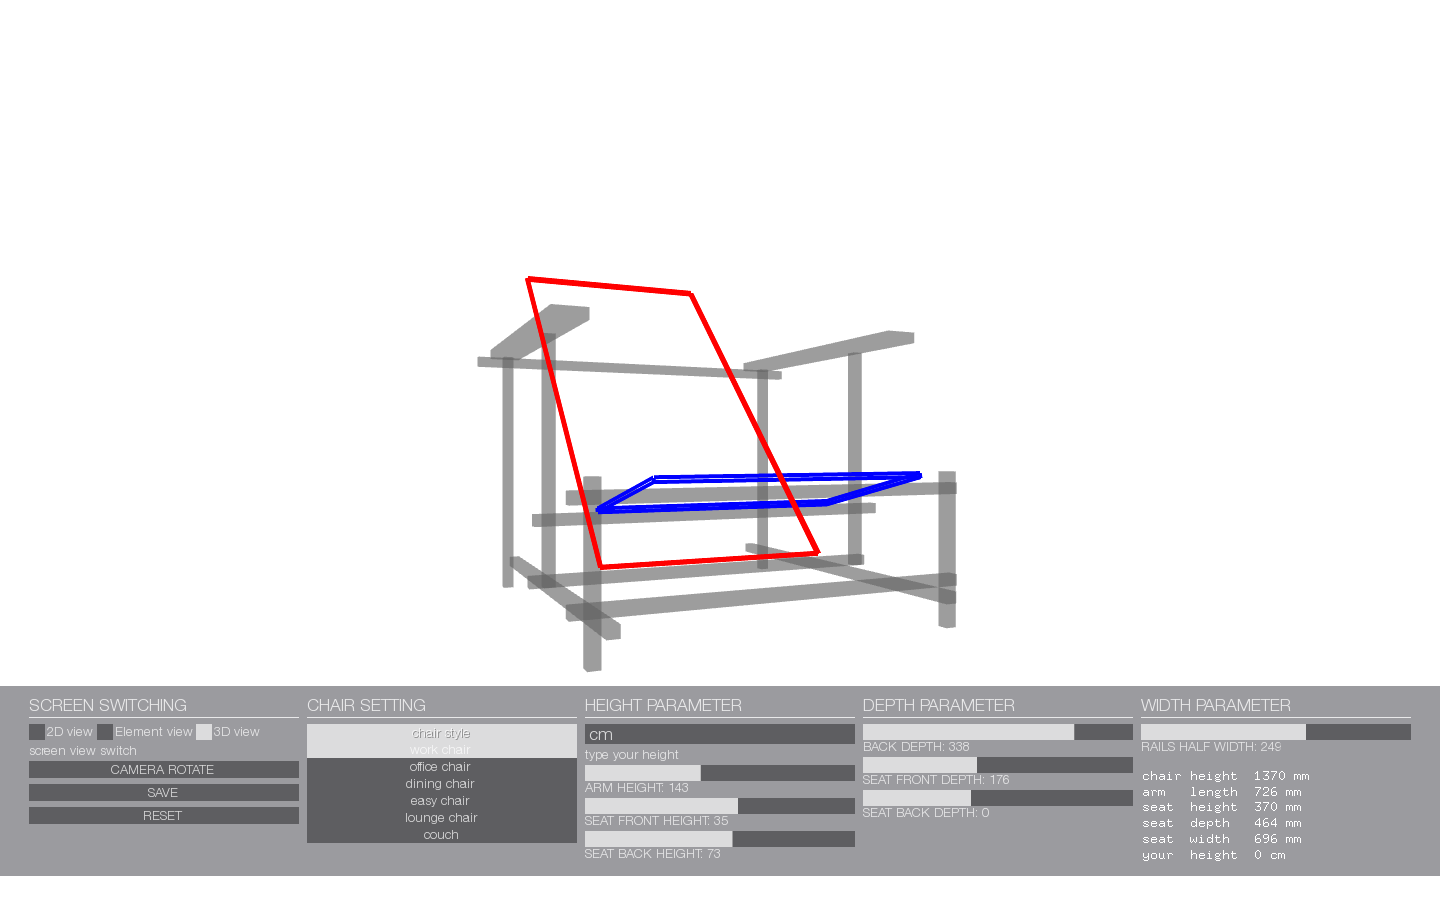
\includegraphics[width=\columnwidth]{images/03.png}
                        \caption{chairGenerator UI}
                        \label{fig:01}
                    \end{figure}
                \end{column}
                \begin{column}{0.50\textwidth}
                    \begin{block}{手順}
                        \begin{itemize}
                            \item パラメーターをスライドする
                            \item SAVEボタンを押してパスデータを保存する
                            \item レーザーカッターやショップボットで切る
                        \end{itemize}
                    \end{block}
                \end{column}
            \end{columns}
        \end{frame}

        \begin{frame}
            \frametitle{NormalBoxTool}
            \tiny
            \begin{columns}[c]
                \begin{column}{0.50\textwidth}
                    \begin{figure}[htb]
                        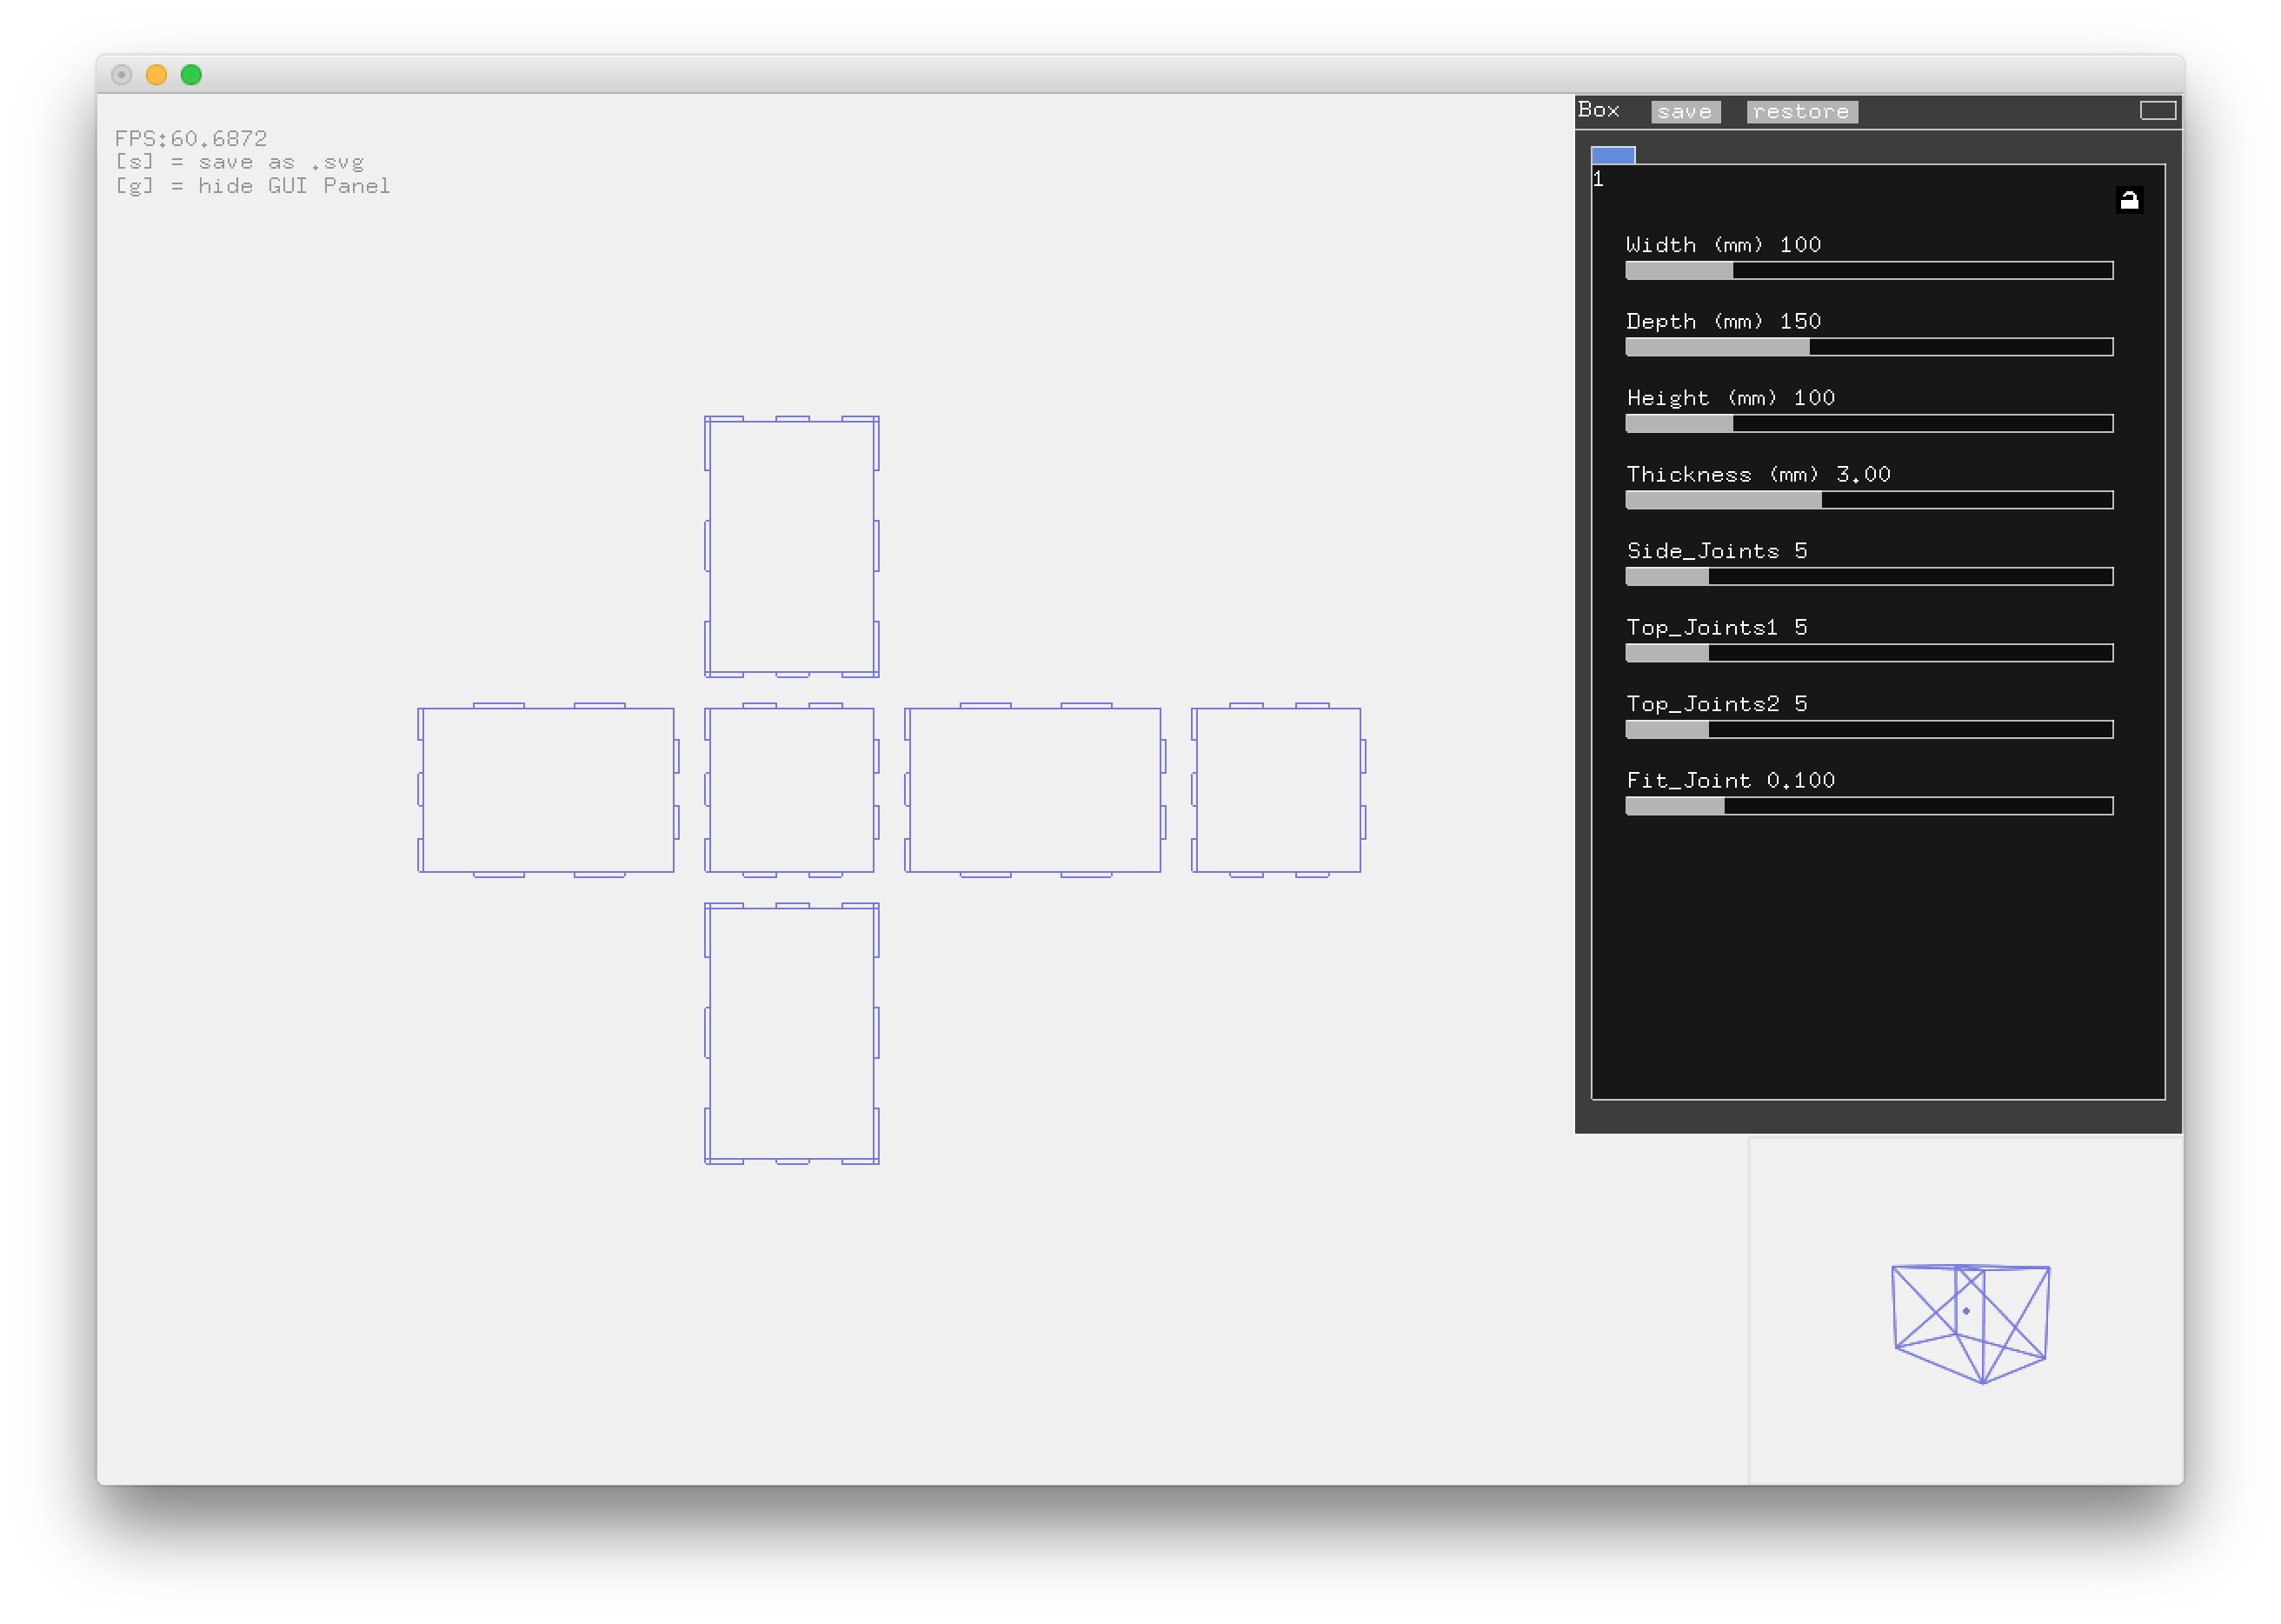
\includegraphics[width=\columnwidth]{images/04.png}
                        \caption{NormalBoxTool UI}
                        \label{fig:01}
                    \end{figure}
                \end{column}
                \begin{column}{0.50\textwidth}
                    \begin{block}{手順}
                        \begin{itemize}
                            \item パラメータをスライドする
                            \item SAVEボタンを押してパスデータを保存する
                            \item レーザーカッターやショップボットで切る
                            \item http://www.instructables.com/id/CuttingBoxTool-How-to-make-a-box-of-various-sizes-/
                        \end{itemize}
                    \end{block}
                \end{column}
            \end{columns}
        \end{frame}

        \begin{frame}
            \frametitle{}
                \begin{figure}[htb]
                    
\includegraphics[width=100mm]{images/05.png}
                    \caption{parayu}
                    \label{fig:03}
                \end{figure}
        \end{frame}

    \section{作例}
        \begin{frame}
            \frametitle{作例}
            \begin{block}{NormalBoxToolの例}
                \begin{itemize}
                    \item http://scottallen.ws/work/zogaku-at-nxpc-live-vol-23-kata
                    \item http://spring.scottallen.ws/
                \end{itemize}
            \end{block}
        \end{frame}

\end{document}


